\documentclass[a4paper,12pt]{article}
\usepackage[english,polish]{babel}
\usepackage{polski}
\usepackage{underscore}
\usepackage[utf8]{inputenc}
\usepackage{graphicx}
\usepackage{tabulary}
\usepackage{array}
\newcommand{\HRule}{\rule{\linewidth}{0.5mm}}

\setlength\fboxsep{1pt}
\setlength\fboxrule{0pt}
\def \tscale {0.3}

\begin{document}

\begin{titlepage}
	\begin{center}
		
\includegraphics[width=0.4\textwidth]{../data/logo} \\[1cm]
		\textsc{\LARGE Technika Mikroprocesorowa} \\[0.8cm]
		\HRule \\[0.4cm]
		{ \huge \bfseries Gesture Processing Library} \\[0.4cm]
		\HRule \\[1.5cm]
	\end{center}
	\begin{minipage}{0.4\textwidth}
		\begin{flushleft} \large
		\emph{Autorzy:} \\
		Michał \textsc{Janiec} \\
		Bartosz \textsc{Polnik}
		\end{flushleft}
	\end{minipage}
\end{titlepage}
\thispagestyle{empty}

\tableofcontents

\section{Temat} \ \\[0.1cm]
\indent Stworzenie niskopoziomowej biblioteki do przetwarzania gestów, dedykowanej dla mikroprocesorów jedno-układowych.

\section{Cel} \ \\[0.1cm]
\indent Celem projektu jest przede wszystkim stworzenie ww. biblioteki pozwalającej na wygodne korzystanie z technologi multi-touch na różnorodnych urządzeniach. Ponadto utworzona zostanie aplikacja na platformę Android służąca zaprezentowaniu działania biblioteki. Jej zadaniem będzie odczytywanie gestów wykonanych przez użytkownika i wyświetlanie ich nazw.

\section{Opis zagadnienia} \ \\[0.1cm]
\indent Zadaniem biblioteki będzie odczytywanie gestów z urządzenia dotykowego. Biblioteka będzie periodycznie odczytywać stan urządzenia (wejście biblioteki). Na tej podstawie będzie rozpoznawać ruchy, które będzie dopasowywać do listy gestów. Po rozpoznaniu gest informacja o wykonanym geście zostanie umieszczona w kolejce gestów (wyjście biblioteki). Użytkownik biblioteki powinien periodycznie sprawdzać czy coś pojawiło się w kolejce i samodzielnie przetwarzać jej zawartość. Gesty będą dodawane do biblioteki w czasie kompilacji. Biblioteka zostanie napisana w języku C bez użycia zewnętrznych bibliotek.



\section{Lista gestów} \ \\[0.1cm]
\indent W celu uniknięcia niejednoznaczności proponujemy anglojęzyczne nazwy gestów.\\

\begin{tabulary}{\linewidth}{|>{\bf}c|c|C|C|}
\hline	\textbf{Nazwa}&\textbf{Rysunek}&\textbf{Opis}&\textbf{Parametry}\\ \hline 
	
     Tap & 
	\fbox{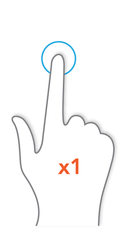
\includegraphics[scale=\tscale]{../data/Tap}} & 
		Pojedyncze stuknięcie w multi-touch. & 	Pozycja (x,y)  \\ \hline
	 
	 Double Tap & \fbox{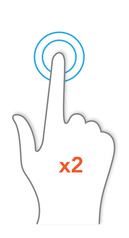
\includegraphics[scale=\tscale]{../data/DoubleTap}} & 
	 	Szybkie podwójne stuknięcie w multi-touch. & Pozycja (x,y)  \\ \hline
	 	
	 Press & \framebox[7em]{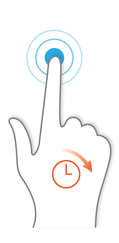
\includegraphics[scale=\tscale]{../data/Press}} &
	 	Stuknięcie i przytrzymanie palca przez dłuższy czas. & 	Pozycja(x,y) \\ \hline
	 	
	 Move & \fbox{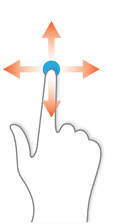
\includegraphics[scale=\tscale]{../data/Move}} &
	 	Przesunięcie palca w dowolnym kierunku. & Pozycja(x,y) Pozycja(x,y) \\ \hline
	 	
	 Rotate & \fbox{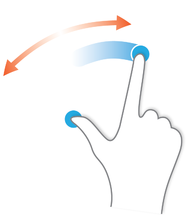
\includegraphics[scale=\tscale]{../data/Rotate}} &
	 	Obrót w lewo lub w prawo. & Left/Right Obrót, (kąt) \\ \hline
	 
	 Flick & \fbox{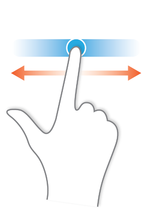
\includegraphics[scale=\tscale]{../data/Flick}} &
	 	Przesunięcie palca w lewo lub prawo i puszczenie. &	Left/Right, Pozycja(x,y) \\ \hline
	 	
\end{tabulary}

\begin{tabulary}{\linewidth}{|>{\bf}C|c|C|C|}
\hline	\textbf{Nazwa}&\textbf{Rysunek}&\textbf{Opis}&\textbf{Parametry}\\ \hline 

	 Scroll & 
\fbox{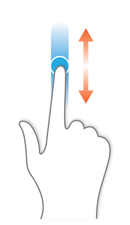
\includegraphics[scale=\tscale]{../data/Scroll}} &
	 	Przesunięcie palca w górę lub w dół i puszczenie. &	Up/Down, Pozycja(x,y) \\ \hline
	 
	 Zoom & \framebox[7em]{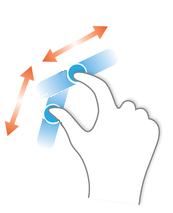
\includegraphics[scale=\tscale]{../data/Zoom}} &
	 	Przybliżenie lub oddalenie palca wskazującego i kciuka do siebie. &	In/Out, Przybliżenie (liczba) \\ \hline
	 
	 Two Finger Scroll & \fbox{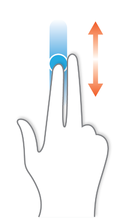
\includegraphics[scale=\tscale]{../data/TwoFingerScroll}} &
	 	Przesunięcie dwóch palców równolegle w górę lub w dół. & Up/Down, Pozycja(x,y) \\ \hline
		
\end{tabulary}

\section{Implementacja}
\subsection{gp_Main.h}
Udostępnia podstawowe funkcje realizowane przez bibliotekę
\subsubsection{Gesture definitions} Zmienne zawierają szczegółowe informacje o wykonanym ruchu

\begin{itemize}
\item \textit{gpOutputGesture_tap}\quad gp_TapData
\item \textit{gpOutputGesture_press}\quad gp_PressData
\item \textit{gpOutputGesture_flick}\quad gp_FlickData
\item \textit{gpOutputGesture_move}\quad gp_MoveData
\item \textit{gpOutputGesture_rotation}\quad gp_RotationData
\item \textit{gpOutputGesture_scroll}\quad gp_ScrollData
\item \textit{gpOutputGesture_zoom}\quad gp_ZoomData
\item \textit{gpOutputGesture_two_finger_scroll}\quad gp_TwoFingerScrollData
\item \textit{gpOutputGesture_two_finger_tap}\quad gp_TwoFingerTapData
\end{itemize}
\subsubsection{Data structures}
\textsf{gpRecognizeContext} \\ \indent Przechowuje informacje o aktualnie wykonywanym ruchu
	\begin{itemize}
		\item \textit{gpVector* finger1}\quad przechowuje zbiór współrzędnych wykonywanego ruchu dla pierwszego palca
		\item \textit{gpVector* finger2}\quad przechowuje zbiór współrzędnych wykonywanego ruchu dla drugiego palca
		\item \textit{gpByte fingers}\quad przechowuje ilość placów biorących udział w ruchu
		\item \textit{gpInt firstTime}\quad przechowuje czas pierwszego dotknięcia ekranu w aktualnym ruchu
	\end{itemize}
\ \\
\subsubsection{Functions}
\mbox{\textsf{gpVoid gpRecognize(gpMotionEvent* event)}} \\ \indent Odpowiada za rozpoznanie gestu
	\begin{itemize}
		\item \textit{gpMotionEvent* event}\quad event do przetworzenia
	\end{itemize}

 \ \\
\mbox{\textsf{gpBool gpTryTap(gpMotionEvent* event, gpRecognizeContext* context)}} \\ \indent Sprawdza, czy aktualnie skończony ruch to tap
	\begin{itemize}
		\item \textit{gpMotionEvent* event}\quad ostatni otrzymany event związany z ruchem
		\item \textit{gpRecognizeContext* context}\quad kontekst związany z ruchem
	\end{itemize}

 \ \\
\mbox{\textsf{gpBool gpTryPress(gpMotionEvent* event, gpRecognizeContext* context)}} \\ \indent Sprawdza, czy aktualnie skończony ruch to press
	\begin{itemize}
		\item \textit{gpMotionEvent* event}\quad ostatni otrzymany event związany z ruchem
		\item \textit{gpRecognizeContext* context}\quad kontekst związany z ruchem
	\end{itemize}

 \ \\
\mbox{\textsf{gpBool gpTryFlick(gpMotionEvent* event, gpRecognizeContext* context)}} \\ \indent Sprawdza, czy aktualnie skończony ruch to flick
	\begin{itemize}
		\item \textit{gpMotionEvent* event}\quad ostatni otrzymany event związany z ruchem
		\item \textit{gpRecognizeContext* context}\quad kontekst związany z ruchem
	\end{itemize}

 \ \\
\mbox{\textsf{gpBool gpTryRotation(gpMotionEvent* event, gpRecognizeContext* context)}} \\ \indent Sprawdza, czy aktualnie skończony ruch to rotation
	\begin{itemize}
		\item \textit{gpMotionEvent* event}\quad ostatni otrzymany event związany z ruchem
		\item \textit{gpRecognizeContext* context}\quad kontekst związany z ruchem
	\end{itemize}

 \ \\
\mbox{\textsf{gpBool gpTryScroll(gpMotionEvent* event, gpRecognizeContext* context)}} \\ \indent Sprawdza, czy aktualnie skończony ruch to scroll
	\begin{itemize}
		\item \textit{gpMotionEvent* event}\quad ostatni otrzymany event związany z ruchem
		\item \textit{gpRecognizeContext* context}\quad kontekst związany z ruchem
	\end{itemize}

 \ \\
\mbox{\textsf{gpBool gpTryZoom(gpMotionEvent* event, gpRecognizeContext* context)}} \\ \indent Sprawdza, czy aktualnie skończony ruch to zoom
	\begin{itemize}
		\item \textit{gpMotionEvent* event}\quad ostatni otrzymany event związany z ruchem
		\item \textit{gpRecognizeContext* context}\quad kontekst związany z ruchem
	\end{itemize}

 \ \\
\mbox{\textsf{gpBool gpTryTwoFingerScroll(gpMotionEvent* event, gpRecognizeContext* context)}} \\ \indent Sprawdza, czy aktualnie skończony ruch to two finger scroll
	\begin{itemize}
		\item \textit{gpMotionEvent* event}\quad ostatni otrzymany event związany z ruchem
		\item \textit{gpRecognizeContext* context}\quad kontekst związany z ruchem
	\end{itemize}

 \ \\
\mbox{\textsf{gpBool gpTryTwoFingerTap(gpMotionEvent* event, gpRecognizeContext* context)}} \\ \indent Sprawdza, czy aktualnie skończony ruch to two finger tap
	\begin{itemize}
		\item \textit{gpMotionEvent* event}\quad ostatni otrzymany event związany z ruchem
		\item \textit{gpRecognizeContext* context}\quad kontekst związany z ruchem
	\end{itemize}

 \ \\
 
Warto zauważyć brak funkcji sprawdzającej, czy aktualnie skończony ruch to move. Wynika to z faktu, iż rozpoznawanie takiego ruchu następuje na bieżąco i informacja o tym ruchu dostępna jest nie tylko po otrzymaniu akcji dotyczącej oderwania ostatniego palca.

\subsection{gp_Alloc.h}
Odpowiada za zarządzanie pamięcią
\subsubsection{Constants}
\begin{itemize}
\item \textit{gpAlloc_MAX_MEM\quad 1000000}\qquad przechowuje rozmiar bufora pamięci tymczasowej
\end{itemize}
\subsubsection{Functions}
\mbox{\textsf{gpVoid* gpAlloc_alloc(gpInt size)}} \\ \indent Przydziela pamięć z bufora
	\begin{itemize}
		\item \textit{gpInt size}\quad ilość jednostek pamięci do przydzielenia
	\end{itemize}

 \ \\
\mbox{\textsf{gpVoid gpAlloc_free(gpVoid* ptr)}} \\ \indent Zwalnia poprzednio przydzieloną z bufora pamięć
	\begin{itemize}
		\item \textit{gpVoid* ptr}\quad wskaźnik na początek zaalokowanej poprzednio pamięci
	\end{itemize}

 \ \\
\mbox{\textsf{gpVoid gpAlloc_copy(gpVoid* from, gpVoid* to, gpInt size)}} \\ \indent Przekopiowuje dane pomiędzy from do to. Nie przydziela pamięci.
	\begin{itemize}
		\item \textit{gpVoid* from}\quad źródło danych do przeniesienia
		\item \textit{gpVoid* to}\quad lokacja do której dane mają być przeniesione
		\item \textit{gpInt size}\quad ilość jednostek do przeniesienia
	\end{itemize}

 \ \\

\subsection{gp.h}
Zawiera użyteczne include'y plików nagłówkowych z folderu base
\subsection{gp_bool.h}
Definiuje podstawowe aliasy na wartości typu logicznego
\subsubsection{Constants}
\begin{itemize}
\item \textit{false\quad 0}\qquad
\item \textit{true\quad 1}\qquad
\end{itemize}

\subsection{gp_point.h}
Zawiera funkcje i struktury dotyczące punktu
\subsubsection{Data structures}
\textsf{gpPoint} \\ \indent Reprezentacja punktu
	\begin{itemize}
		\item \textit{gpFloat x}\quad współrzędna x
		\item \textit{gpFloat y}\quad współrzędna y
	\end{itemize}
\ \\
\subsubsection{Functions}
\mbox{\textsf{gpFloat gpPoint_distance(gpPoint* a, gpPoint* b)}} \\ \indent Oblicza dystans pomiędzy dwoma punktami w przestrzeni
	\begin{itemize}
		\item \textit{gpPoint* a}\quad wskaźnik na pierwszy punkt
		\item \textit{gpPoint* b}\quad wskaźnik na drugi punkt
	\end{itemize}

 \ \\
\mbox{\textsf{gpFloat gpPoint_distance2(gpPoint* a, gpPoint* b)}} \\ \indent Oblicza kwadrat odległości pomiędzy punktami
	\begin{itemize}
		\item \textit{gpPoint* a}\quad wskaźnik na pierwszy punkt
		\item \textit{gpPoint* b}\quad wskaźnik na drugi punkt
	\end{itemize}

 \ \\
\mbox{\textsf{gpPoint gpPoint_init(gpFloat x, gpFloat y)}} \\ \indent Tworzy punkt o zadanych współrzędnych
	\begin{itemize}
		\item \textit{gpFloat x}\quad współrzędna x
		\item \textit{gpFloat y}\quad współrzędna y
	\end{itemize}

 \ \\

\subsection{gp_printf.h}
Zawiera funkcie pomocne przy debugowaniu na platformie android

\subsection{gp_types.h}
Definiuje abstrakcję na typy zależne od platformy
\subsubsection{Data types}
\begin{itemize}
\item \textit{typedef void gpVoid}
\item \textit{typedef char gpBool}
\item \textit{typedef unsigned char gpUByte}
\item \textit{typedef signed char gpByte}
\item \textit{typedef unsigned short gpUWord}
\item \textit{typedef signed short gpWord}
\item \textit{typedef unsigned long gpUInt}
\item \textit{typedef signed long gpInt}
\item \textit{typedef char gpChar}
\item \textit{typedef char* gpString}
\item \textit{typedef long gpFloat}
\end{itemize}
\subsubsection{Constants}
\begin{itemize}
\item \textit{null\quad ((gpVoid*)(0))}\qquad pomocna reprezentacja wskaźnika o wartości nieokreślonej
\end{itemize}

\subsection{gp_vector.h}
Opisuje abstrakcyjną kolekcję i operacje na niej
\subsubsection{Data structures}
\textsf{gpVector}	\\ \indent Kolekcja
	\begin{itemize}
		\item \textit{gpVoid** data}\quad wskaźnik na pierwszy element kolekcji
		\item \textit{gpInt capacity}\quad aktualna pojemność kolekcji
		\item \textit{gpInt size}\quad aktualny rozmiar kolekcji
	\end{itemize}
\ \\
\subsubsection{Functions}
\mbox{\textsf{gpVoid gpVector_init(gpVector* self)}} \\ \indent Inicjalizuje kolekcję (alokuje pamięć na jej elementy)
	\begin{itemize}
		\item \textit{gpVector* self}\quad wskaźnik na zaalokowaną kolekcję
	\end{itemize}

 \ \\
\mbox{\textsf{gpVoid gpVector_destroy(gpVector* self)}} \\ \indent Zwalnia pamięć zajmowaną przez kolekcję
	\begin{itemize}
		\item \textit{gpVector* self}\quad wskaźnik na kolekcję
	\end{itemize}

 \ \\
\mbox{\textsf{gpInt gpVector_getSize(gpVector* self)}} \\ \indent Zwraca rozmiar kolekcji
	\begin{itemize}
		\item \textit{gpVector* self}\quad wskaźnik na kolekcję
	\end{itemize}

 \ \\
\mbox{\textsf{gpVoid* gpVector_at(gpVector* self, gpInt index)}} \\ \indent Zwraca wskaźnik na element kolekcji
	\begin{itemize}
		\item \textit{gpVector* self}\quad wskaźnik na kolekcję
		\item \textit{gpInt index}\quad numer wskaźnika do elementu do zwrócenia
	\end{itemize}

 \ \\
\mbox{\textsf{gpVoid gpVector_clean(gpVector* sefl)}} \\ \indent Czyści zawartość kolekcji
	\begin{itemize}
		\item \textit{gpVector* sefl}\quad wskaźnik na kolekcję
	\end{itemize}

 \ \\
\mbox{\textsf{gpVoid gpVector_pushBack(gpVector* self, gpVoid* what, gpInt size)}} \\ \indent Dokłada element na koniec kolekcji
	\begin{itemize}
		\item \textit{gpVector* self}\quad wskaźnik na kolekcję
		\item \textit{gpVoid* what}\quad wskaźnik na element do dołożenia
		\item \textit{gpInt size}\quad rozmiar elementu dokładanego
	\end{itemize}

 \ \\
\mbox{\textsf{gpVoid gpVector_popBack(gpVector* self, gpVoid* where, gpInt size)}} \\ \indent Usuwa ostatni element z kolekcji
	\begin{itemize}
		\item \textit{gpVector* self}\quad wskaźnik na kolekcję
		\item \textit{gpVoid* where}\quad wskaźnik na miejsce w pamięci, w które ma być przeniesiony ostatni element kolekcji
		\item \textit{gpInt size}\quad rozmiar elementu kolekcji
	\end{itemize}

 \ \\

\subsection{gp_gestures_parameters.h}
Opisuje parametry dotyczące tolerancyjności w wykrywaniu ruchów
\subsubsection{Constants}
\begin{itemize} 
\item \textit{GP_TAP_MAX_TIME\quad 40}\qquad maksymalny czas tap'a
\item \textit{GP_TAP_MAX_MOVE\quad gpMkFloat("12")}\qquad maksymalne odchylenie ruchu dla tapa
\item \textit{GP_ROTATION_DIST_PARAM\quad gpMkFloat("0.35")}\qquad maksymalna różnica odległości (proporcjonalnie do odległości początkowej)
\item \textit{GP_ROTATION_MIN_ANGLE\quad gpMkFloat("9")}\qquad minimalny kąt obrotu (stopnie)
\item \textit{GP_ROTATION_MAX_MOVE\quad gpMkFloat("35")}\qquad maksymalne odchylenie podczas wykonywania rotacji
\item \textit{GP_TAP_PRESS_MOVE\quad gpMkFloat("10")}\qquad maksymalnie odchylenie dla długiego przyciśnięcia
\item \textit{GP_SCROLL_MIN_LEN\quad gpMkFloat("20")}\qquad minimalna odległość dla ruchu scroll
\item \textit{GP_FLICK_MIN_LEN\quad gpMkFloat("15")}\qquad minimalna odległość dla ruchu flick
\item \textit{GP_TWO_FINGER_TAP_MAX_DIST\quad gpMkFloat("60")}\qquad maksymalna odległość dla two finger tap
\item \textit {GP_NOTATIME\quad -1}\qquad Wartość oznaczająca że czas jest nie ustawiony. 
\item \textit{GP_ZOOM_MIN_CHANGE\quad gpMkFloat("10")}\qquad minimalna odległość dla zoom
\end{itemize}

\subsection{gp_gestures_results.h}
Definiuje stałe pomocne przy rozpoznawaniu kierunków ruchu
\subsubsection{Constants}
\begin{itemize}
\item \textit{GP_SCROLL_DOWN\quad true}\qquad definiuje kierunek w dół
\item \textit{GP_SCROLL_UP\quad false}\qquad definiuje kierunek w górę
\item \textit{GP_FLICK_LEFT\quad false}\qquad definiuje ruch w lewo
\item \textit{GP_FLICK_RIGHT\quad true}\qquad definiuje ruch w prawo
\item \textit{GP_ZOOM_IN\quad true}\qquad definiuje przybliżenie
\item \textit{GP_ZOOM_OUT\quad false}\qquad definiuje oddalenie
\end{itemize}

\subsection{gp_MotionEvent.h}
Określa znacznie kodu akcji w evencie
\subsubsection{Constants}
\begin{itemize}
\item \textit{GP_ME_ACTION_DOWN\quad 0}\qquad początek ruchu
\item \textit{GP_ME_ACTION_MOVE\quad 2}\qquad ruch po ekranie
\item \textit{GP_ME_ACTION_POINTER_1_DOWN\quad 5}\qquad opuszczenie pierwszego palca na ekran
\item \textit{GP_ME_ACTION_POINTER_1_UP\quad 6}\qquad podniesienie pierwszego palca
\item \textit{GP_ME_ACTION_POINTER_2_DOWN\quad 261}\qquad opuszczenie drugiego palca
\item \textit{GP_ME_ACTION_POINTER_2_UP\quad 262}\qquad podniesienie drugiego palca
\item \textit{GP_ME_ACTION_UP\quad 1}\qquad koniec ruchu
\end{itemize}

\subsection{gp_OutputGesture.h}
Zawiera struktury reprezentujące dodatkowe informacje o ruchu
\subsubsection{Data structures}
\textsf{gpOutputGesture_two_finger_scroll} \\ \indent Reprezentuje two finger scroll
	\begin{itemize}
		\item \textit{gpFloat x}\quad przesunięcie poziome
		\item \textit{gpFloat y}\quad przesunięcie pionowe
		\item \textit{gpBool direction}\quad kierunek przewinięcia
	\end{itemize}
\ \\
\textsf{gpOutputGesture_zoom} \\ \indent Reprezentuje zoom
	\begin{itemize}
		\item \textit{gpBool direction}\quad kierunek
		\item \textit{gpFloat magnification}\quad stosunek odległości
	\end{itemize}
\ \\
\textsf{gpOutputGesture_scroll} \\ \indent Reprezentuje scroll
	\begin{itemize}
		\item \textit{gpFloat x}\quad przesunięcie poziome
		\item \textit{gpFloat y}\quad przesunięcie pionowe
		\item \textit{gpBool direction}\quad kierunek przewinięcia
	\end{itemize}
\ \\
\textsf{gpOutputGesture_flick} \\ \indent Reprezentuje flick
	\begin{itemize}
		\item \textit{gpFloat x}\quad przemieszczenie poziome
		\item \textit{gpFloat y}\quad przemieszczenie pionowe
		\item \textit{gpBool direction}\quad kierunek przemieszczenia
	\end{itemize}
\ \\
\textsf{gpOutputGesture_rotation} \\ \indent Reprezentuje rotation
	\begin{itemize}
		\item \textit{gpBool direction}\quad informacja, czy kąt jest dodatni, czy ujemny
		\item \textit{gpFloat angle}\quad kąt obrotu
	\end{itemize}
\ \\
\textsf{gpOutputGesture_move} \\ \indent Reprezentuje przesunięcie
	\begin{itemize}
		\item \textit{gpFloat x}\quad początkowa współrzędna x
		\item \textit{gpFloat y}\quad początkowa współrzędna y
		\item \textit{gpFloat begx}\quad końcowa współrzędna x
		\item \textit{gpFloat begy}\quad końcowa współrzędna y
	\end{itemize}
\ \\
\textsf{gpOutputGesture_press} \\ \indent Reprezentuje press
	\begin{itemize}
		\item \textit{gpFloat x}\quad współrzędna x
		\item \textit{gpFloat y}\quad współrzędna y
	\end{itemize}
\ \\
\textsf{gpOutputGesture_tap} \\ \indent Reprezentuje tap
	\begin{itemize}
		\item \textit{gpFloat x}\quad współrzędna x
		\item \textit{gpFloat y}\quad współrzędna y
	\end{itemize}
\ \\
\textsf{gpOutputGesture_two_finger_tap} \\ \indent Reprezentuje two finger tap
	\begin{itemize}
		\item \textit{gpFloat x}\quad współrzędna x
		\item \textit{gpFloat y}\quad współrzędna y
	\end{itemize}
\ \\

\subsection{gp_Math.h}
Zawiera deklarację zaimplementowanych funkcji oraz stałych
\subsubsection{Constants}
\begin{itemize}
\item \textit{GP_FLOAT_BASE\quad 10000}\qquad część liczby przeznaczona na miejsca dziesiętne
\item \textit{gpMath_EPSILION\quad 10}\qquad epsilon 
\item \textit{gpMath_PI\quad 31416}\qquad PI
\item \textit{gpMath_2PI\quad 62832}\qquad dwukrotność PI
\item \textit{gpMath_PI2\quad 15708}\qquad połowa liczy PI
\item \textit{gpMath_PI4\quad 7854}\qquad PI przez 4
\item \textit{gpMath_PI6\quad 5236}\qquad PI przez 6
\item \textit{gpMath_E\quad 27183}\qquad E
\item \textit{gpMath_1\quad 10000}\qquad 1
\item \textit{gpMath_2\quad 20000}\qquad 2
\item \textit{gpMath_3\quad 30000}\qquad 3
\item \textit{gpMath_SINPI4\quad 7071}\qquad sinus PI przez 4
\item \textit{gpMath_0\quad 0}\qquad 0
\end{itemize}
\subsubsection{Functions}
\mbox{\textsf{gpFloat gpMul(gpFloat a, gpFloat b)}} \\ \indent Mnoży dwie liczy stałopozycyjne
	\begin{itemize}
		\item \textit{gpFloat a}\quad mnożna
		\item \textit{gpFloat b}\quad mnożnik
	\end{itemize}

 \ \\
\mbox{\textsf{gpFloat gpDiv(gpFloat a, gpFloat b)}} \\ \indent Dzieli dwie liczy stałopozycyjne
	\begin{itemize}
		\item \textit{gpFloat a}\quad dzielna
		\item \textit{gpFloat b}\quad dzielnik
	\end{itemize}

 \ \\
\mbox{\textsf{gpFloat gpSub(gpFloat a, gpFloat b)}} \\ \indent odejmuje dwie liczy stałopozycyjne
	\begin{itemize}
		\item \textit{gpFloat a}\quad odjemna
		\item \textit{gpFloat b}\quad odjemnik
	\end{itemize}

 \ \\
\mbox{\textsf{gpFloat gpAdd(gpFloat a, gpFloat b)}} \\ \indent Dodaje dwie liczy stałopozycyjne
	\begin{itemize}
		\item \textit{gpFloat a}\quad składnik
		\item \textit{gpFloat b}\quad składnik
	\end{itemize}

 \ \\
\mbox{\textsf{gpFloat gpNeg(gpFloat a)}} \\ \indent Zwraca liczbę przeciwną do danej liczy stałopozycyjnej
	\begin{itemize}
		\item \textit{gpFloat a}\quad operand
	\end{itemize}

 \ \\
\mbox{\textsf{gpInt gpMath_MinInt()}} \\ \indent Zwraca mniejszą z liczb typu gpInt
	\begin{itemize}
		\item \textit{gpFloat a}\quad operand
		\item \textit{gpFloat b}\quad operand
	\end{itemize}

 \ \\
\mbox{\textsf{gpByte gpMath_Sign(gpFloat x)}} \\ \indent Zwraca signum liczby
	\begin{itemize}
		\item \textit{gpFloat x}\quad operand
	\end{itemize}

 \ \\
\mbox{\textsf{gpFloat gpMath_Abs(gpFloat a)}} \\ \indent Zwraca wartość bezwzględną liczby
	\begin{itemize}
		\item \textit{gpFloat a}\quad operand
	\end{itemize}

 \ \\
\mbox{\textsf{gpFloat gpMath_Square(gpFloat a)}} \\ \indent Zwraca kwadrat liczby
	\begin{itemize}
		\item \textit{gpFloat a}\quad operand
	\end{itemize}

 \ \\
\mbox{\textsf{gpFloat gpMath_Sqrt(gpFloat a)}} \\ \indent Zwraca pierwiastek liczy
	\begin{itemize}
		\item \textit{gpFloat a}\quad operand
	\end{itemize}

 \ \\
\mbox{\textsf{gpFloat gpMath_Exp(gpFloat a)}} \\ \indent Zwraca E podniesione do potęgi a
	\begin{itemize}
		\item \textit{gpFloat a}\quad operand
	\end{itemize}

 \ \\
\mbox{\textsf{gpFloat gpMath_PowI(gpFloat base, gpInt exp)}} \\ \indent Potęguje
	\begin{itemize}
		\item \textit{gpFloat base}\quad liczba do podniesienia
		\item \textit{gpInt exp}\quad wykładnik
	\end{itemize}

 \ \\
\mbox{\textsf{gpFloat gpMath_Sin(gpFloat x)}} \\ \indent Oblicza sinus
	\begin{itemize}
		\item \textit{gpFloat x}\quad kąt w radianach
	\end{itemize}

 \ \\
\mbox{\textsf{gpFloat gpMath_Cos(gpFloat x)}} \\ \indent Oblicza kosinus
	\begin{itemize}
		\item \textit{gpFloat x}\quad kąt podany w radianach
	\end{itemize}

 \ \\
\mbox{\textsf{gpFloat gpMath_Tan(gpFloat x)}} \\ \indent Oblicza tangens
	\begin{itemize}
		\item \textit{gpFloat x}\quad kąt podany w radianach
	\end{itemize}

 \ \\
\mbox{\textsf{gpFloat gpMath_ATan2(gpFloat x, gpFloat y)}} \\ \indent Oblicza wartość bliższego kąta pomiędzy punktem, a osią x
	\begin{itemize}
		\item \textit{gpFloat x}\quad współrzędna x
		\item \textit{gpFloat y}\quad współrzędna y
	\end{itemize}

 \ \\
\mbox{\textsf{gpFloat gpMath_ASin(gpFloat x)}} \\ \indent Oblicza arcus-sinus
	\begin{itemize}
		\item \textit{gpFloat x}\quad kąt w radianach
	\end{itemize}

 \ \\
\mbox{\textsf{gpFloat gpMath_ACos(gpFloat x)}} \\ \indent Oblicza arcus-kosinus
	\begin{itemize}
		\item \textit{gpFloat x}\quad kąt podany w radianach
	\end{itemize}

 \ \\
\mbox{\textsf{gpFloat gpMath_ATan(gpFloat x)}} \\ \indent Oblicza arcus-tangens
	\begin{itemize}
		\item \textit{gpFloat x}\quad kąt podany w radianach
	\end{itemize}

 \ \\
\mbox{\textsf{gpFloat gpMath_MinFloat(gpFloat a, gpFloat b)}} \\ \indent Zwraca mniejszą z liczb
	\begin{itemize}
		\item \textit{gpFloat a}\quad operand
		\item \textit{gpFloat b}\quad operand
	\end{itemize}

 \ \\
\mbox{\textsf{gpFloat gpMath_MaxFloat(gpFloat a, gpFloat b)}} \\ \indent Zwraca większą z liczb
	\begin{itemize}
		\item \textit{gpFloat a}\quad operand
		\item \textit{gpFloat b}\quad operand
	\end{itemize}

 \ \\
\mbox{\textsf{gpBool gpMath_Equals(gpFloat a, gpFloat b)}} \\ \indent Porównuje dwie liczby
	\begin{itemize}
		\item \textit{gpFloat a}\quad operand
		\item \textit{gpFloat b}\quad operand
	\end{itemize}

 \ \\
\mbox{\textsf{gpInt gpMath_Int(gpFloat a)}} \\ \indent Zamienia liczbę stałopozycyjną na całkowitą
	\begin{itemize}
		\item \textit{gpFloat a}\quad liczba stałopozycyjna
	\end{itemize}

 \ \\
\mbox{\textsf{gpFloat gpMath_FloatI(gpInt a)}} \\ \indent Zwraca liczbę całkowitą na stałopozycyjną
	\begin{itemize}
		\item \textit{gpInt a}\quad liczba całkowita
	\end{itemize}

 \ \\
\mbox{\textsf{gpFloat gpMath_AngleToAzimut(gpPoint a, gpPoint b)}} \\ \indent Oblicza kąt skierowany między punktami
	\begin{itemize}
		\item \textit{gpPoint a}\quad pierwszy punkt
		\item \textit{gpPoint b}\quad drugi punkt
	\end{itemize}

 \ \\
\mbox{\textsf{gpFloat gpMkFloat(gpString x)}} \\ \indent Tworzy liczbę stałopozycyjną z napisu
	\begin{itemize}
		\item \textit{gpString x}\quad napis
	\end{itemize}

 \ \\

\section{Pliki}
\begin{itemize}
\item \textit{gp_Main.h}\quad project_c\textbackslash BaseProject\textbackslash Include
\item \textit{gp_Alloc.h}\quad project_c\textbackslash BaseProject\textbackslash Include\textbackslash Alloc
\item \textit{gp.h}\quad project_c\textbackslash BaseProject\textbackslash Include\textbackslash Base
\item \textit{gp_bool.h}\quad project_c\textbackslash BaseProject\textbackslash Include\textbackslash Base
\item \textit{gp_point.h}\quad project_c\textbackslash BaseProject\textbackslash Include\textbackslash Base
\item \textit{gp_printf.h}\quad project_c\textbackslash BaseProject\textbackslash Include\textbackslash Base
\item \textit{gp_types.h}\quad project_c\textbackslash BaseProject\textbackslash Include\textbackslash Base
\item \textit{gp_vector.h}\quad project_c\textbackslash BaseProject\textbackslash Include\textbackslash Base
\item \textit{gp_gestures_parameters.h}\quad project_c\textbackslash BaseProject\textbackslash Include\textbackslash Gestures
\item \textit{gp_gestures_results.h}\quad project_c\textbackslash BaseProject\textbackslash Include\textbackslash Gestures
\item \textit{gp_MotionEvent.h}\quad project_c\textbackslash BaseProject\textbackslash Include\textbackslash InOut
\item \textit{gp_OutputGesture.h}\quad project_c\textbackslash BaseProject\textbackslash Include\textbackslash InOut
\item \textit{gp_Math.h}\quad project_c\textbackslash BaseProject\textbackslash Include\textbackslash Math
\item \textit{gp_Main.c}\quad project_c\textbackslash BaseProject\textbackslash Source
\item \textit{gp_Alloc.c}\quad project_c\textbackslash BaseProject\textbackslash Source\textbackslash Alloc
\item \textit{gp.c}\quad project_c\textbackslash BaseProject\textbackslash Source\textbackslash Base
\item \textit{gp_point.c}\quad project_c\textbackslash BaseProject\textbackslash Source\textbackslash Base
\item \textit{gp_printf.c}\quad project_c\textbackslash BaseProject\textbackslash Source\textbackslash Base
\item \textit{gp_vector.c}\quad project_c\textbackslash BaseProject\textbackslash Source\textbackslash Base
\item \textit{gp_flick.c}\quad project_c\textbackslash BaseProject\textbackslash Source\textbackslash Gestures
\item \textit{gp_gestures.c}\quad project_c\textbackslash BaseProject\textbackslash Source\textbackslash Gestures
\item \textit{gp_press.c}\quad project_c\textbackslash BaseProject\textbackslash Source\textbackslash Gestures
\item \textit{gp_rotation.c}\quad project_c\textbackslash BaseProject\textbackslash Source\textbackslash Gestures
\item \textit{gp_scroll.c}\quad project_c\textbackslash BaseProject\textbackslash Source\textbackslash Gestures
\item \textit{gp_tap.c}\quad project_c\textbackslash BaseProject\textbackslash Source\textbackslash Gestures
\item \textit{gp_zoom.c}\quad project_c\textbackslash BaseProject\textbackslash Source\textbackslash Gestures
\item \textit{gp_MotionEvent.c}\quad project_c\textbackslash BaseProject\textbackslash Source\textbackslash InOut
\item \textit{gp_Math.c}\quad project_c\textbackslash BaseProject\textbackslash Source\textbackslash Math
\end{itemize}

\end{document}